You will use the ultrasonic echo sensor to determine the distance to an object.

\subsection{Theory of Operation}

The ultrasonic echo sensor has a simple interface.
If your program places a logic-high signal on the sensor's \texttt{Trig} (``trigger'') pin for 10\textmu s and then drop it to logic-low, then the device will emit a short burst of ultrasound.
The device will then raise the \texttt{Echo} pin's logic level to high.
If there is a nearby object, the ultrasound will reflect off of it, and the sensor will detect the echo.
After detecting the echo, the device will drop the \texttt{Echo} pin's logic level to low.
If no echo is received, then the device will eventually time-out and drop the \texttt{Echo} pin's logic level to low.
After affording the device a quiescent period, the cycle can be repeated.

Various datasheets\footnote{
    \url{https://cdn.sparkfun.com/datasheets/Sensors/Proximity/HCSR04.pdf}}$^,$\footnote{\url{https://web.eece.maine.edu/~zhu/book/lab/HC-SR04\%20User\%20Manual.pdf}}$^,$\footnote{\url{https://www.handsontec.com/dataspecs/HC-SR04-Ultrasonic.pdf}
}\ differ slightly in a few particulars.
Some describe the time-out period as 36ms, others 38ms.
Some describe the quiescent period as at least 10ms after the \texttt{Echo} pin's logic drops low; others recommend at least 60ms after the \texttt{Echo} pin's logic goes high.
The datasheets generally agree that under typical conditions, the device will be able to detect an echo from a $0.5\mathrm{m}^2$ target within 4~meters of the sensor.
One datasheet suggests that under some conditions, this distance may be as great as 5~meters.\footnote{
    During testing of the sample solution, sometimes objects 250cm away couldn't always be reliably detected; at other times I was able to detect objects up to 320cm away.
}

If your program measures the time between the \texttt{Echo} pin's logic going high and subsequently going low, then it knows how long the ultrasound travelled to the object and back again.
The classical relationship $distance = speed \times time$ requires that we know how fast the ultrasound travels.

The speed of sound depends on the medium it travels through and the temperature of that medium.
We will assume the medium is air, and that its temperature is 70\degree~Fahrenheit (21.1\degree~Celsius), the temperature that Avery Hall's thermostats are often set at.
The speed of sound for 70\degree\ air is $348.8\frac{m}{s}$.\footnote{
    \url{https://www.weather.gov/epz/wxcalc_speedofsound}
} As the distance is required to be calculated in centimeters, let us convert the speed of sound's units accordingly:

\[
    \frac{343.8 m}{1 s} \times \frac{100 cm}{1 m} \times \frac{1 s}{1,000,000 \mu s} = 0.034,38 \frac{cm}{\mu s}
\]

\subsection{Practical Considerations}

We want to avoid floating point calculations, which are computationally expensive on an 8-bit microcontroller.
Even if we reduced the denominator to period of the system clock, the shortest amount of time that can be measured, the speed of sound is $0.550,08 \frac{cm}{0.0625\mu s}$ and would still require floating point arithmetic.

%\[
%    \frac{1 s}{343.8 m} \times \frac{m}{100 cm} \times \frac{1,000,000 \mu s}{1 s} \approx 29 \frac{\mu s}{cm}
%\]

In real-number arithmetic, multiplying the speed of sound by a constant non-zero finite value and by time, and dividing by the same constant value, will produce the same distance as if the speed of sound were multiplied by time.
In bit-limited integer arithmetic, the same is true \textit{if} the original speed were an integer, \textit{if} the product doesn't overflow, and \textit{if} all multiplications occur before division.
Because we're treating the speed of sound as a constant, and the conversion factor is also a constant, part of the multiplication can occur at compile-time, ensuring that both the run-time multiplier and multiplicand are integers.
Normally, integer division on an 8-bit microcontroller is only slightly more desirable than floating point arithmetic;
however, if the constant factor is a power of two, then the division can be accomplished with a bitshift operation.

If we also recognize that for every meter the object is from the sensor, the ultrasound must travel two meters (1m to the object plus 1m back to the sensor), then we can determine the multiplicand to multiply by the measured time:

\[
    \frac{343.8 m~\mathrm{\mbox{\tiny sound~travel}}}{1 s} \times \frac{1 m~\mathrm{\mbox{\tiny object~distance}}}{2 m~\mathrm{\mbox{\tiny sound~travel}}} \times \frac{100 cm}{1 m} \times \frac{1 s}{1,000,000 \mu s} \times \frac{2^{20}}{2^{20}} \approx \frac{18,025 cm~\mathrm{\mbox{\tiny object~distance}}}{\mu s} \div 2^{20}
\]

Any object within range of the sensor will have a measured time that, when multiplied by 18,025, will yield a product that fits in a 32-bit \lstinline{long}.
(Convince yourself of this by multiplying the greatest time-out period -- 38,000\textmu s -- by 18,025.)

The other practical timing consideration is that the Arduino function \function{micros()} reports the number of microseconds since power-up to within 4\textmu s.
By properly configuring a timer, we can measure time more precisely.
Unfortunately, if you look at the possible prescalers \textcolor{green}{in Section~6 of the Cow Pi's datasheet}, you will see that we cannot set a timer to beat every microsecond.
We can, however, set a timer to beat every half-microsecond with a prescaler of 8:

\[
    \left(16,000,000\frac{cycle}{second} \times \frac{1}{8}\frac{beat}{cycle} \times \frac{1~second}{1,000,000~microseconds}\right)^{-1} = \frac{\frac{1}{2}\mu s}{beat}
\]

We now adjust the expression to compute the object's distance:

\[
    distance = time_{\mu s} \times \frac{18,025 cm}{\mu s} \div 2^{20} = time_{\frac{1}{2}\mu s} \times \frac{18,025 cm}{\frac{1}{2}\mu s} \div 2^{21}
\]

There is also a practical consideration with respect to the sensor itself.
Sound isn't particularly directional.
The horns surrounding the ultrasonic transducers help to limit the ``beam width,'' but only to a degree.
Pointing the sensor straight down an otherwise empty hallway, you will probably still detect a reflection from the walls to either side.\footnote{
    If you're feeling nerdy, you could use right-angle trigonometry to determine the ``beam width'' --
    point the sensor straight at a wall to determine how far away from it you are (the ``opposite''), then point the sensor parallel to the wall and take a reading (the hypoteneuse).
    Divide the ``opposite'' by the hypoteneuse and take the arcsin -- the resulting value is the angle from straigth-ahead to how far to the right/left the sensor will detect a reflection.
}

\subsection{Examining the Starter Code}

The \function{initialize_sensor()} function is where you'll place any alarm-related code that needs to be run once when the program starts.
The \function{manage_sensor()} function is where you'll place any alarm-related code that needs to run with every iteration of the program's main loop.
You will, of course, add code outside these functions too: an interrupt service routine for a timer, an interrupt handler for the distance sensor, and possibly helper functions.

\subsection{Single-Pulse Operation} \label{subsec:distanceSinglePulseOperation}

Create a variables to:
\begin{itemize}
    \item indicate whether an object has been detected
    \item indicate the object's distance (if the object is detected)
    \item indicate the object's rate of approach (this will only be useful in Normal Operation mode)
\end{itemize}
Be sure to declare them not only in \textit{sensor.c} (without the \lstinline{extern} modifier) but also in \textit{shared\_variables.h} (with the \lstinline{extern} modifier).
In \function{initialize_sensor()}, initialize the object detection variable to indicate that an object has not been detected.

A fully-correct implementation of Single-Pulse Operation mode has the alarm chirp if an object is detected closer than the threshold range (Requirement~\ref{spec:singlePulseOperation}).
For now, your focus will be on determining the distance to an object.

Using the ``Timers'' section of the Cow Pi datasheet,\footnote{
    \url{https://cow-pi.readthedocs.io/en/latest/microcontroller.html\#timers}
}
place code in \function{initialize_sensor()} to configure Timer1 to produce an \textbf{overflow} interrupt every 32,768\textmu s, using the ``Normal'' mode.
Place in \function{initialize_sensor()} code to enable that interrupt.

Create a state machine for the sensor that can be ``ready,'' ``active-listening,'' ``active-detected,'' and ``quiescent.''
Initialize it to be ``ready.''

\begin{figure}[h]
    \centering
    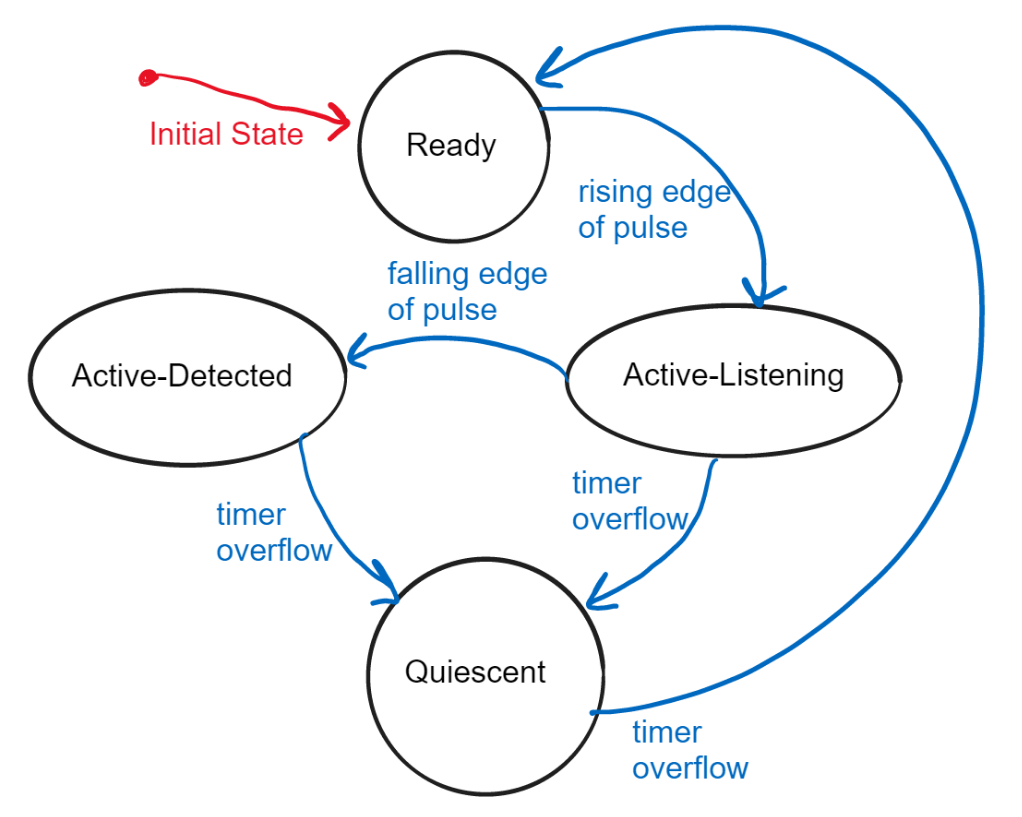
\includegraphics[width=3in]{sensorStateMachine}
    \caption{\label{fig:sensorStateMachine} State machine describing the control of the distance sensor.
        See Appendix~\ref{sec:phantom} for an alternative state machine.}
\end{figure}

Use the \function{ISR} macro to create an interrupt service routine in \textit{sensor.c} for that interrupt.
Leave the ISR's body empty for now.

Create a temporarily-empty interrupt handler in \textit{sensor.c} that will be used to detect the rising and falling edge of the pulse. %one for actions to be taken when the sensor emits its ultrasound pulse, and one for actions to be taken when the sensor receives an echo.
Don't forget to pre-declare this functions above \function{initialize_sensor()}.
Place in \function{initialize_sensor()} code to register the handler for a CHANGE on Arduino pin~D3.

\paragraph{Initiate a Pulse}
Place code in \function{manage_sensor()} that, whenever a ping is requested (see Section~\ref{subsec:readPushbutton}), will:
\begin{itemize}
    \item First, set Arduino pin~D2 to logic-high
    \item Then, set the variable indicating that a ping is requested to \lstinline{false}
    \item Next, delay for 10\textmu s
    \item Finally, set pin~D2 to logic-low
\end{itemize}

Several microseconds later, the sensor will emit its ultrasound pulse and raise its \texttt{Echo} line to logic-high.

\paragraph{Handle the Start of a Pulse}
In the function that you registered to handle the pulse edges on pin~D3, you want to keep track of whether the interrupt handler was triggered for a rising or falling edge.
While you \textit{could} do so by checking the logic level on pin~D3, you can also assume that rising and falling edges alternate --
you will never have two rising edges in a row, and you will never have two falling edges in a row.

If the interrupt handler was triggered for a rising edge, you want to start the process of determining exactly how much time passes between emitting the pulse and receiving the echo.
\begin{itemize}
    \item First, using its memory-mapped I/O \lstinline{struct}, set TIMER1's counter to 0
    \item Then, place the sensor in its ``active-listening'' state
\end{itemize}

Two things will happen in the next 38 (or fewer) milliseconds: the signal on pin~D3 will fall to logic-low, and TIMER1 will overflow.
Whichever happens first, the signal falling low or the \textit{real} TIMER1 overflow, will tell us whether there's an object.

\paragraph{Handle the End of a Pulse}
If the signal on pin~D3 falls to logic-low first, then it's because there's an object that reflected the ultrasound pulse.

If the interrupt handler was triggered for a falling edge, and if the sensor is ``active-listening,'' then you want to capture the information needed to compute the distance.
\begin{itemize}
    \item First, copy the value of TIMER1's counter into a \lstinline{volatile} global variable -- this is the number of half-microseconds between the pulse emission and the echo's return
    \item Then, place the sensor in its ``active-detected'' state
\end{itemize}

\paragraph{Handle Timer Overflow}

If the TIMER1 overflows before the signal on pin~D3 falls low, then there is not an object within detectable range.
The sensor will time-out after 36,000--38,000\textmu s, and TIMER1 will overflow after $65,536 \div 2 = 32,768\mu \mathrm{s}$.
Any object whose echo might have been detected after this must be at least $65,536 \times 18,025 \div 2^{21} \approx 563\mathrm{cm}$ away, but no datasheets suggest that the sensor can detect objects more than 500cm away.

If the sensor is ``active-listening'' then no object was detected:
\begin{itemize}
    \item First, indicate that an object has not been detected
    \item Then, place the sensor in its ``quiescent'' state
\end{itemize}

On the other hand, if the sensor is ``active-detected'' then an object was detected:
\begin{itemize}
    \item First, indicate that an object has been detected
    \item Then, place the sensor in its ``quiescent'' state
\end{itemize}

As noted above, some describe the quiescent period as at least 10ms after the \texttt{Echo} pin's logic drops low; others recommend at least 60ms after the \texttt{Echo} pin's logic goes high.
We shall allow 65.536ms after the \texttt{Echo} pin's logic goes high, which is guaranteed to satisfy both.
32,768\textmu s after \texttt{Echo} pin's logic went high, the timer overflowed and you placed the sensor in its ``quiescent'' state.
32,768\textmu s after that, it will overflow again.

If the sensor is ``quiescent'' when the timer ISR is triggered:
\begin{itemize}
    \item Place the sensor in its ``ready'' state
\end{itemize}

\paragraph{Compute and Display the Distance}

Add code to the \function{manage_sensor()} function that, if an object has been detected, computes the distance (as a whole number of centimeters) to the object.
Display the clearly-labeled distance on the display module.
Now add code to the \function{manage_sensor()} function that, if an object has \textit{not} been detected, displays on the display module a clear indication that there is no detected object.
As a small optimization, you might have your code make these updates only when the sensor is ``quiescent.''

\vspace{0.5cm}

Test your code.
I recommend that you place your Cow~Pi on top of its food-container carrying case, or some other object, to reduce the likelihood of the sensor receiving an echo from your worktable.

\vspace{0.5cm}

Most of the work to configure the alarm for Single-Pulse Operation takes place in Section~\ref{subsec:soundSinglePulseOperation}.
You will finish implementing Single-Pulse Operation in Section~\ref{subsec:integrationSpeedSinglePulseOperation} by integrating the detection code from Section~\ref{subsec:distanceSinglePulseOperation} with the alarm code from Section~\ref{subsec:soundSinglePulseOperation}.
This will require small changes to the code.
